\chapter{Theoretical background}\label{chaptertheoreticalbackground}
\section{Introduction}
This book presents an overview of the clause structure of German Sign Language (\textit{Deutsche Gebärdensprache}, DGS), an SOV language used in Germany. The main claim is that scopal relations are mapped onto the body in a systematic way in this language, an idea first introduced in \citet{bross2017scope}. I will show that the clausal domains with highest scope, to be more precise all CP functions (i.\,e., all categories above T) are expressed non-manually with the face, starting with the eyebrows and finally switching to the lower face. Lower, IP-internal aspectual categories (called the `outer aspects')\is{outer aspect} are produced manually using adverbs. The same is true for IP-internal modal categories which are expressed using manual modal verb signs. I will show that these manual signs systematically occur pre-verbally, i.\,e., overtly scope from left to right (with the verb being linearly to the right of the scope-taking element). This relation then switches to a right-to-left concatenation strategy when it comes to Voice adverbs (e.\,g., \textsc{well}). Finally, I will show that the lower, VoiceP-internal aspects (called the `inner aspects')\is{aspect}\is{inner aspect} are systematically produced by manipulating the movement path of the verb sign. 

In this first chapter on the theoretical background of the present study, I will introduce the two theoretical frameworks I will follow, namely Generative Grammar (to be more precise Minimalism) and the Cartographic approach to syntax (Section \ref{theoryintroa} and \ref{theoryintrob}). Finally, in Section \ref{hypotheses} the main hypotheses are introduced.% and in Section \ref{methods}, I will discuss data elicitation. Finally, I will give a brief overview of the content of the remainder of the book (Section \ref{outlinesection}).

%\section{Theoretical Underpinnings}\label{theoryintro}


\section{Generative Grammar and the Minimalist Program}\label{theoryintroa}
The goal of the present and the section to follow is to introduce the two theoretical frameworks which underlie the current study. First, I will briefly outline the main claims of the Generative Grammar and the Minimalist program and then, in the next section, discuss the basics of Cartographic syntax. 

Generative Grammar is a grammatical theory in which the grammar of a language is taken to be a set of rules able to create structures (and only those structures) which are judged to be grammatical by native speakers/hearers/signer of that language. While there have been several different approaches or schools in the history of Generative Grammar, what they all have in common is that they try to model the knowledge of an ideal native signer/speaker which allows her/him to master the language. One of these approaches is called `Minimalism' or the `Minimalist program'. Minimalism is a research program in the tradition of Generative Grammar developed in the early 1990s. It is a syntactic account which tries to model syntax in the most parsimonious, natural, and elegant way while not denying that there may be other (equivalent) ways to model syntax. This means that it is more a research program than a theory: ``$[$M$]$inimalism is not a theory so much as a program for research. $[$\dots $]$ Theories are true or false. Programs are fecund or sterile'' \citep[6]{hornstein2005understanding}.

\subsection{Modeling I-language}\is{I-language}
The goal of the Minimalist framework, as with older frameworks in the Generative tradition, is to model the computational system underlying language. As with its predecessors, the Principles and Parameters Theory and Government and Binding, the core goal of the Minimalist program is to study the tacit linguistic competence, i.\,e., the cognitive system which is able to generate grammatical structures, called `I-language'. The I-language, with `I' standing for \textit{internal}, \textit{intensional}, and \textit{individual}, is understood as a property of the mind/brain of an individual, i.\,e., a state of the mind. This state of the mind can have different manifestations. Before a human being has experienced any linguistic input this state is called the `initial state' and after a human being has acquired a language it is called the `steady state' (i.\,e., the state in which an individual has the knowledge to master a language). Thus, Minimalism, as well as its predecessors, tries to study the I-language, an abstract state of the mind, and not (a set of) concrete utterances which are labeled \is{E-language}`E-language', with `E' standing for \textit{externalized} and \textit{extensional} \citep{chomsky1986barr}.

\subsection{The Idea of the Language Faculty and Universal Grammar}
Humans acquire a language through input which means that there is some (limited) data a child has access to, called `primary linguistic data'. The simplest model to account for the fact that humans are able to acquire a language through this input looks like the one in (\ref{simplemodelug}). This model simply states that any typically developing human being is able to acquire any natural language through primary linguistic data as an input. This input is processed by the individual's brain resulting in acquiring competence in the language. 

\begin{exe}
\ex\label{simplemodelug} Primary linguistic data \ding{212} \fbox{human brain} \ding{212} I-language
\end{exe}

\noindent Since the early days of Generative Grammar, the existence of a set of principles for constructing grammars has been postulated, which is thought to be innate in the form of a modular subsystem, while connected to, but crucially encapsulated from, the general cognitive system. The reason for assuming the existence of this system, called `faculty of language' (or `language faculty'), was that humans are able to effortlessly acquire any human language despite its complexity and despite the fact that the primary linguistic data is quite limited and impoverished in nature. From this, the model in (\ref{simplemodelug}) can be reformulated as in (\ref{simplemodelugb}). According to this view, language acquisition ``is primarily a matter of filling in detail within a structure that is innate'' \citep[39]{chomsky1975reflections}.

\begin{exe}
\ex\label{simplemodelugb} Primary linguistic data \ding{212} \fbox{faculty of language} \ding{212} I-language
\end{exe}

\noindent The theory of the initial state of the faculty of language is called `Universal Grammar' (UG), although the term is widely used with the meaning of this state or the module itself. This means that it was assumed that those abstract grammatical principles which are universal should be regarded as being part of our biological endowment, i.\,e., innate. Although there has been much criticism on the idea that this kind of UG exists (e.\,g., \citealt{evans2009myth}; \citealt{levinson2010time}), it is still clear that indeed much uniformity exists across the languages of the world. This does not only relate to the way that languages are acquired, which is cross-linguistically similar, but also to the possible ways grammars are structured. The main controversy since the beginning of Generative syntax has been the origins of this uniformity and the question of whether an innate faculty of language really exists and what it looks like. 
A logical consequence was to reduce the theoretical machinery. Subsequently, the faculty of language was divided into two parts, the language faculty in the broad (FLB) and the language faculty in the narrow sense (FLN) \citep{hauser2002faculty,fitch2005evolution}. While the original idea of Generative approaches was the existence of a linguistic module totally encapsulated from general cognition, it was now thought that the FLB draws back on resources of general cognition and that the FLN only consists of the basic syntactic mechanisms of (recursive) Merge, i.\,e., of an operation that allows structure building and movements. 

This development did not come out of nowhere, but was the result of two competing forces. On the one hand, Generative linguists (following ideas by \citealt{fodor1975language, jerry1983modularity}) have defended the view of a strictly encapsulated language processing module (with several submodules). On the other hand, cognitive psychologists since the 1990s/2000s developed a diametrically opposed view according to which language is not processed in an amodal, encapsulated  module, but processed in brain areas which are highly interrelated with neural circuitries responsible for motor control and perception. Since then, cognitive psychologists have accumulated a huge body of evidence that lends support to the view that linguistic processing draws back on mechanisms of general cognition, a view called `grounded cognition' or `embodied language processing' (see, for example, \citealt{glenberg2002grounding}; \citealt{pecher2005grounding}; \citealt{barsalou2008grounded}).

\begin{figure}[bt]
\centering
	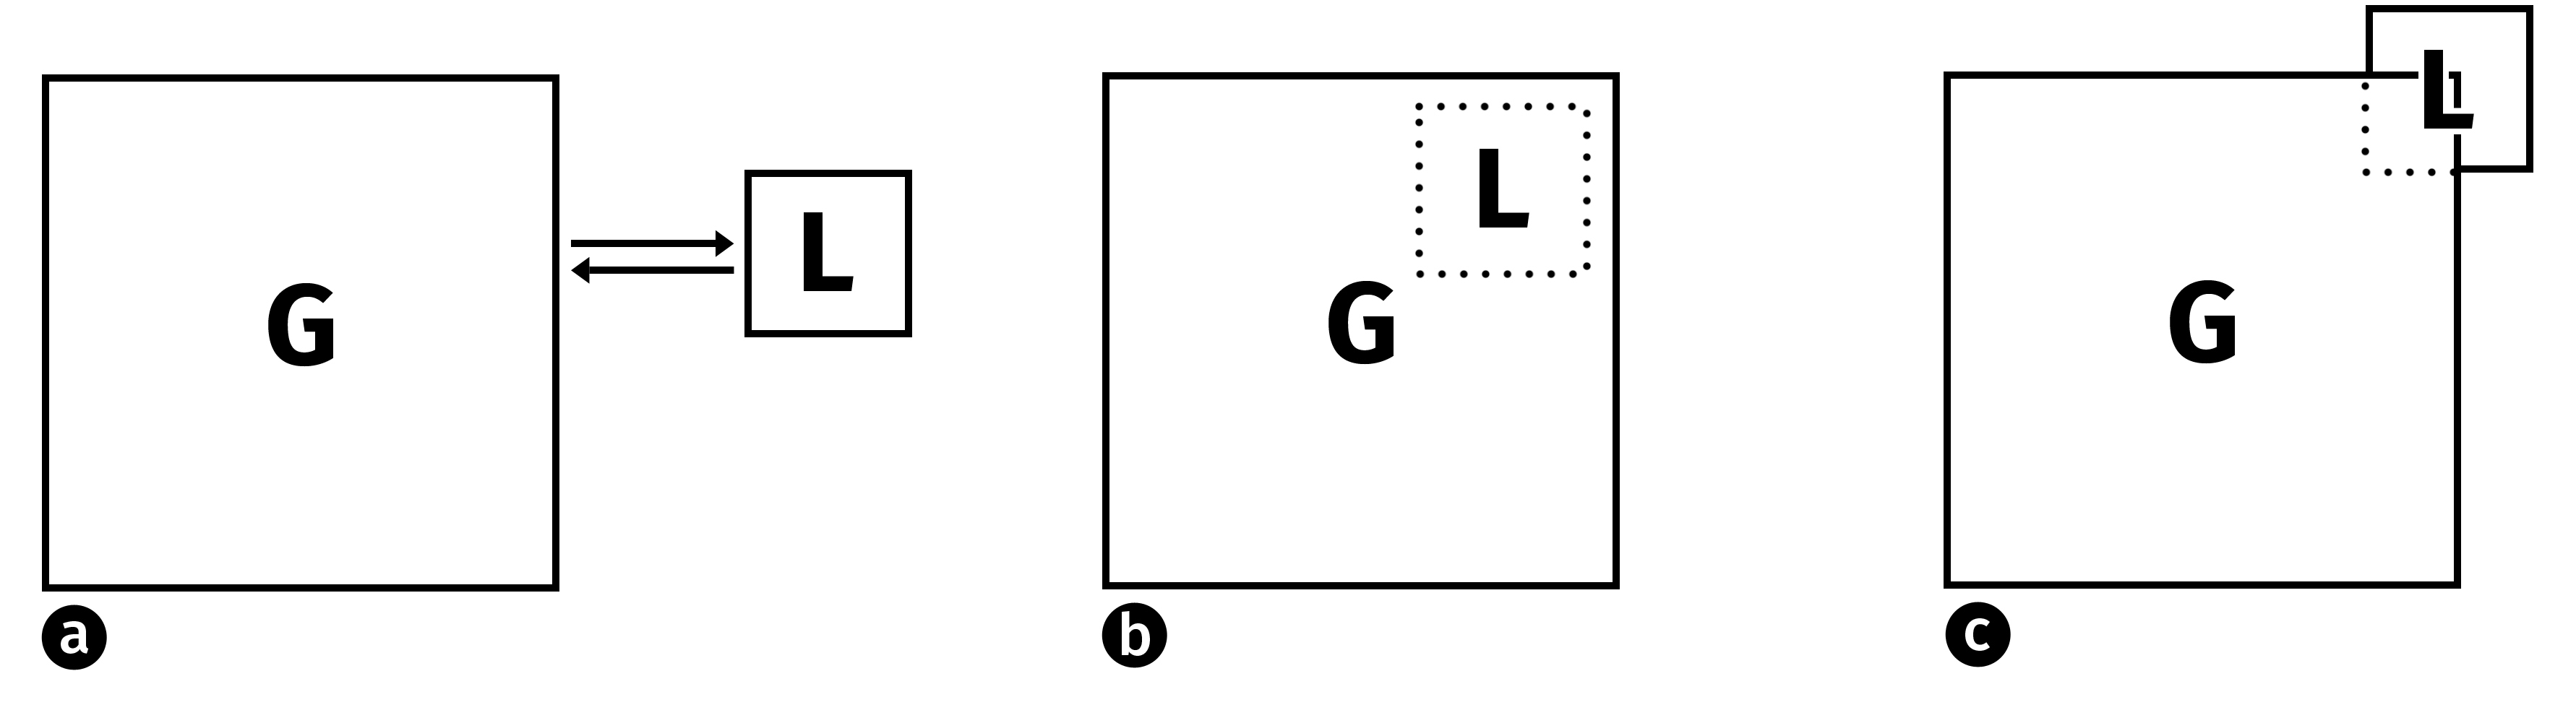
\includegraphics[width=1.0\textwidth]{modelsw.jpg}
	\caption{a) The modular view of language (L) as being an encapsulated and innate module that is separated from general cognition (G); b) Proponents of embodied cognition approaches think of language not as an innate module, but rather as a processing system that draws on general cognitive resources; c) An integrated view.}
	\label{model}
\end{figure}

Thus, according to the modularist view, language is processed in an encapsulated module which is separated by general cognition, as shown in Figure \ref{model}a, while linguistic processing is totally integrated into the general cognition according to embodied language processing approaches, as shown in Figure \ref{model}b.  In a sense, Minimalism is an attempt to bring these two opposing world-views together in claiming that FLN is a separate module and FLB draws back on general cognitive resources, as illustrated in Figure \ref{model}c. This means that both language acquisition and language processing in the adult speaker-hearer/signer rely on two different parts: a specialized language module and general cognition. Thus, while the term `Minimalism' is often understood in a sense that the program tries to minimalize the theoretical machinery used to describe a grammar -- and this is indeed true --, the core meaning is that it is not only this machinery that should be minimal, but the language faculty that is modeled as being biologically minimal (e.\,g., \citealt{sigurdsson2011uniformity}).

\subsection{The Y-model of grammar}
While the basic mechanism of conjoining and manipulating linguistic strings (i.\,e., Merge) is thought of as part of the FLN, there are two systems that play a role in Minimalist approaches being part of general cognition. The first is the sensorimotor system, to be more precise, the articulatory-perceptual system (A-P system) and the second the conceptual-intentional system (C-I system). As these systems need to communicate with the modules responsible for linguistic processing, there is a need for at least two interfaces. These interfaces, i.\,e., the linguistic levels connected to the A-P system and the C-I system respectively, are the Phonological Form (PF) and the Logical Form (LF). While PF is the mental representation of sound/sign, LF is the mental representation of meaning, although in a rather abstract sense as LF is only concerned with the part of meaning which can be derived from structural relationships (in a syntactic tree).
 
\begin{figure}[bt]
\centering
	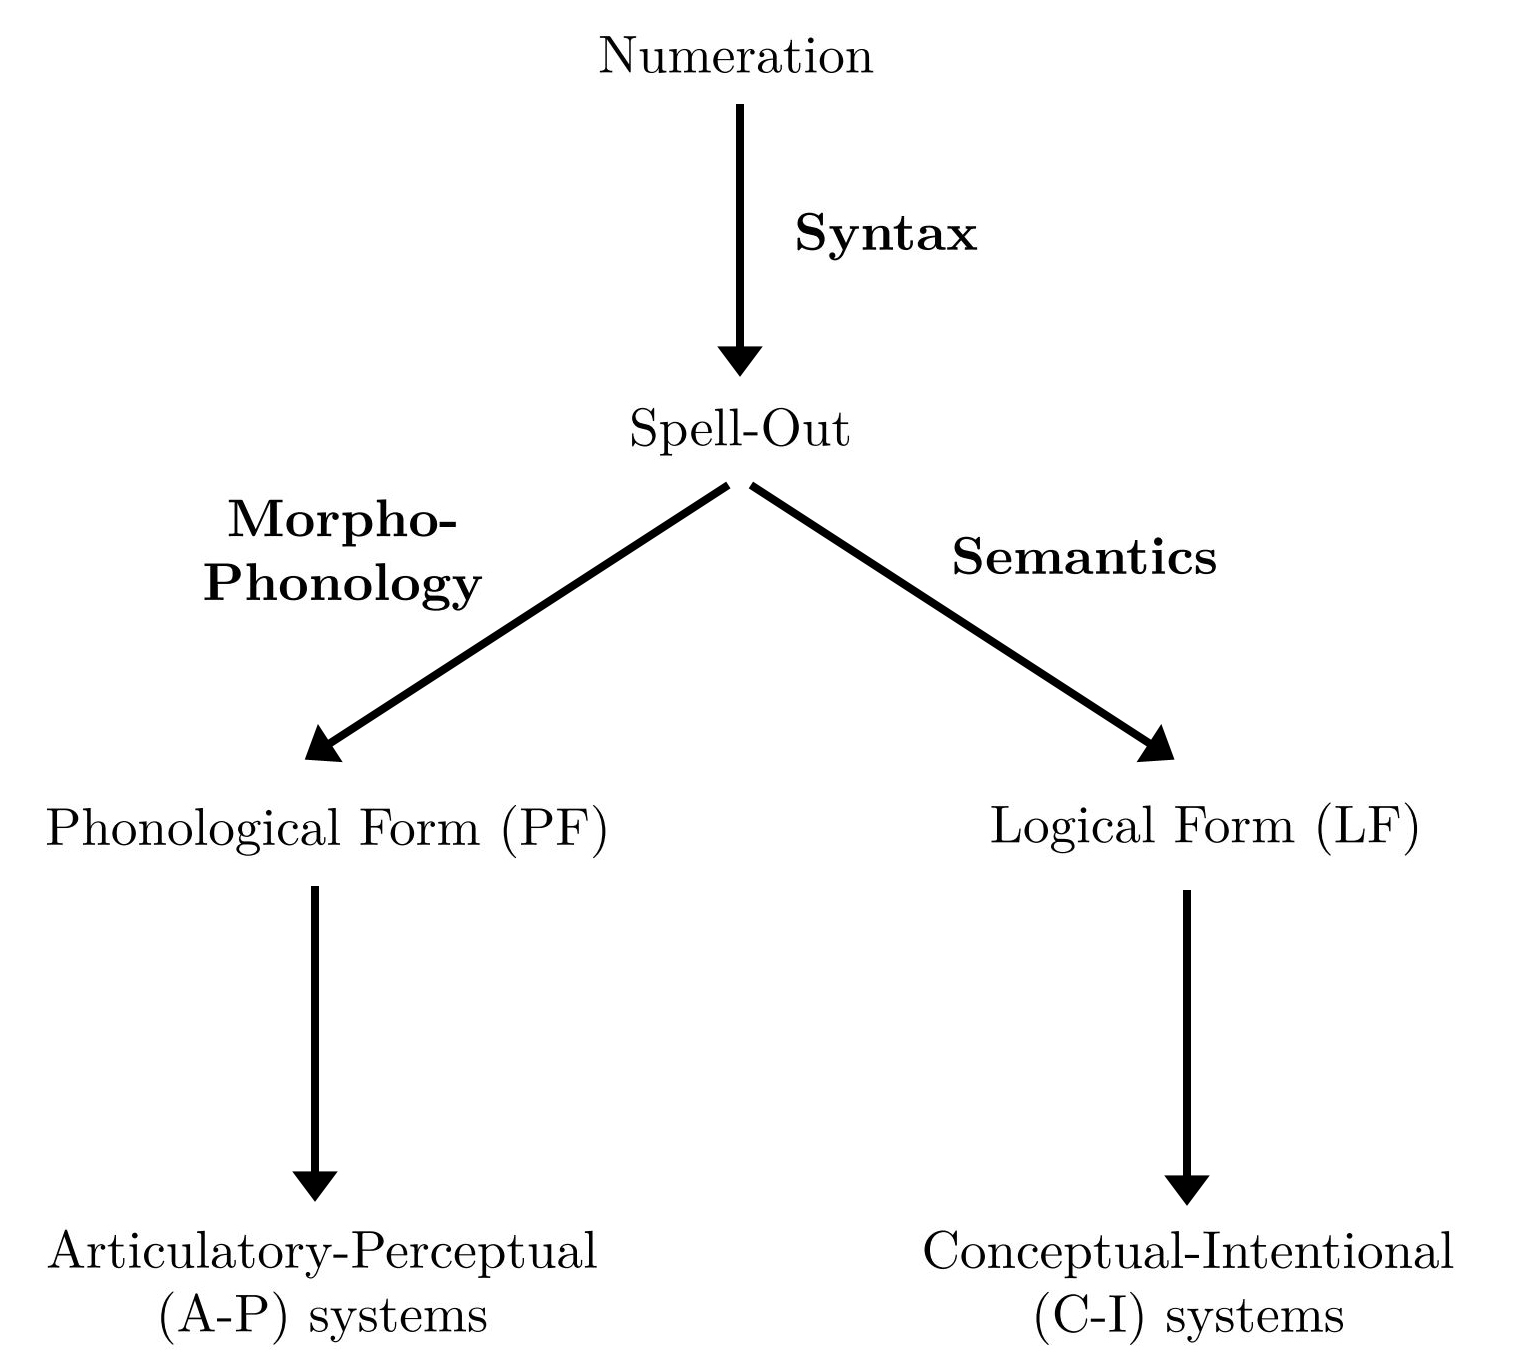
\includegraphics[width=1.0\textwidth]{ymodelsw.jpg}
	\caption{The Y-model of grammar.}
	\label{ymodel}
\end{figure}

The relation between PF and LF (as the interfaces) on the one hand and the A-P and the C-I system on the other are depicted in what is generally known as the `Y-model of grammar' (also called `T-model of grammar'), shown in Figure \ref{ymodel}. The basic idea of this model is that the derivation of a sentence starts by picking out the lexical items needed to construct a sentence (note that the term `lexical item' is used in a very broad sense here as it includes both content and functional elements). This string of lexical items is called the `numeration'. The numeration is handed over into what is called the `workspace of the derivation'. In the workspace, syntactic operations are performed on the numeration, i.\,e., syntactic structure is built via two types of Merge: External Merge combines two elements and Internal Merge (also Remerge or Movement) operates on syntactic objects created via External Merge. This module, labeled `syntax' in the Y-model in Figure \ref{ymodel}, is sometimes called `overt syntax' as the operations carried out in this module produce audible/visible effects in the syntax.

At this point in the derivation, i.\,e., after syntax has produced a syntactic object via External and Internal Merge, the syntactic object is shipped off to the interfaces. This point in the derivation is called `Spell-Out' (note that this is not the point at which something is actually pronounced as the name may suggest). Here, the derivation splits up, as there are syntactic operations which are not visible when pronouncing or signing a sentence. Think of \textit{wh}-\textit{in-situ}-languages in which a \textit{wh}-operator is interpreted as if it were high up in the structure although this is not the case in the actual sentence. To account for this, a module is needed to take care of such operations. This module is labeled `semantics' in Figure \ref{ymodel}. Sometimes this module is also called `covert syntax' as the operations carried out in the module are not overt. Note, again, that semantics or meaning at this point of the derivation only refers to meaning which can be derived from structural relationships (which does, of course, not mean that elements from the derivation having meaning on their own cannot enter this branch). As what is actually pronounced or signed can be different from the LF representation, another branch is needed in which morphological and phonological operations can be carried out. The results of these operations are shipped to the PF interface, as shown in the figure.

\subsection{Features}

The most concrete entity in a derivation as has been sketched so far is a lexical item and the most concrete form of a lexical item is a word. Each word in a language follows it own rules. There is a rule for how to pronounce it, a rule for what the word means, and rules for what the morphological shape of a word looks like in certain environments. These `rules' are called features. Thus, a lexical item consists (at most) of phonological, semantic, and morphosyntactic features -- note that this leaves open the possibility that lexical items without phonological features exist. If we look at morphosyntactic features, it turns out that they come in two flavors. Some features have semantic content and others do not. Take the word \textit{cats} which bears a plural feature (the plural marker /z/ is not the feature itself, but the realization of this feature). This feature has semantic import as it becomes clear that a word like \textit{cats} is referring to several entities. Features of this type are called `interpretable features' as they are interpretable at LF. The terminological counterpart of interpretable features are uninterpretable features which, then, are features which are not interpretable at LF. An example of an uninterpretable feature is Case: In the example in (\ref{casea}), the pronoun \textit{her} is, because of its syntactic position, required to be in objective case. This particular construction does not allow another Case. Nominative Case, for example, is disallowed, as shown in (\ref{caseb}). This is a pure structural requirement and does not directly add anything to the meaning as we can see from the example in (\ref{casec}) which are equal from a semantic perspective, but in this structure only nominative Case is allowed (cf. (\ref{cased})). 

\begin{exe}
\ex\label{case}\begin{xlist}
\ex \textcolor{white}{*}Gökce believes \textit{her} to be smart. \label{casea}
\ex *Gökce believes \textit{she} to be smart. \label{caseb}
\ex \textcolor{white}{*}Gökce believes that \textit{she} is smart. \label{casec}
\ex *Gökce believes that \textit{her} is smart. \label{cased}
\end{xlist}
\end{exe}








\noindent Lexical items are not only specified for features by themselves, but also bear features specifying what features other lexical items should carry in order to be able to Merge with them. Such features are called subcategorization features. Take the lexical item \textit{to} in a construction like \textit{I gave the beer to Felicia} which can, obviously, be Merged with a DP (in this case, the DP \textit{Felicia}). We can thus state that the preposition \textit{to} has an uninterpretable subcategorization feature $[$\textit{u}DP$]$. As the DP \textit{Felicia} bears a matching feature, the features are checked (or valuated) in the derivation and subsequently deleted. The deletion of uninterpretable features is necessary as the derivation would crash if features which are not interpretable at LF enter LF or PF. From this, it becomes clear that features are the driving force of Merge. This is true not only for External Merge, but also for Internal Merge. Thus movement (or Internal Merge) must be motivated in some way and this way is feature checking (or: feature valuation). 

\subsection{The $\overline{\textrm{X}}$ schema}
\is{x schema@$\overline{\textrm{X}}$ schema|(}
As External Merge always combines two lexical items (or more broadly speaking, two syntactic objects) it is an operation which always leads to binary branching structures \citep{kaynel984}. As (External) Merge has been, so far, only defined as an operation which takes two syntactic objects and combines them into a larger syntactic object, Merge is an extremely powerful mechanism which needs to be constrained in order to not overgeneralize. A first constraint on Merge was already introduced with subcategorization features. Another constraint concerns the way the resulting structures look. The way the output (i.\,e., phrases) looks is modeled by the $\overline{\textrm{X}}$ schema (`X-bar schema') which states that all phrases have essentially the same structural skeleton \citep{jackendoff1977x,chomsky1986barr}:\footnote{ Note that some frameworks try to get rid of the $\overline{\textrm{X}}$ schema completely by assuming that all levels of the $\overline{\textrm{X}}$ structure can be read off from structural relationships of the tree geometry created by merge (e.\,g., \citealt{chomsky1995bare}). However, I will not adopt such a bare phrase structure approach\is{bare phrase structure} as the Cartographic framework I am working in traditionally models clausal maps in an $\overline{\textrm{X}}$ format, but nothing hinges on that as I assume that $\overline{\textrm{X}}$ structures and bare phrase structures are compatible and that one representation can be translated into the other.} Phrases are organized around syntactic heads which determine the categorical status of a phrase. Heads may optionally have sisters which themselves are phrases. These sisters are called `complements'. Additionally, heads may have an immediately c-commanding phrase called `specifier' with c-command (constituent command), informally being defined as having a structural relationship of the following form: a node A in a syntactic tree c-commands its sister B and all the descendants of B, i.\,e., all nodes dominated by B. We thus arrive at a structural representation as in (\ref{xbar}). 

\begin{exe}
\ex\label{xbar} 
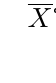
\begin{tikzpicture}[baseline={([yshift={-2.3ex}]current bounding box.north)}, scale=0.90]
\tikzset{level distance=50pt,sibling distance=25pt,every tree node/.style={align=center,anchor=north}}
\Tree [.XP [.SpecXP ] [.{$\overline{\text{X}}$} [.{X\textdegree } ] [.{YP (Complement)} ] ] ] 
\end{tikzpicture}
\end{exe}

\noindent The representation in (\ref{xbar}) tells us that the core of the $\overline{\textrm{X}}$ schema is a head, in this case the head X\textdegree\ (with the little circle being an abbreviation for head). It projects its categorical status to the whole phrase which then is an XP. While there may be more structure built around an XP, the categorical status cannot project any further. For this reason, XPs are also called `maximal projections'. Note that the terms `specifier', `head', and `complement' are purely structural terms which means that it does not matter on which side of the tree any of the three elements are located. Thus, the structure in (\ref{xbarb}) is also in accordance with the $\overline{\textrm{X}}$ schema (as would be structures with a specifier on one and the head on the other side of the tree).

\begin{exe}
\ex\label{xbarb} 
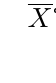
\begin{tikzpicture}[baseline={([yshift={-2.3ex}]current bounding box.north)}, scale=0.90]
\tikzset{level distance=50pt,sibling distance=25pt,every tree node/.style={align=center,anchor=north}}
\Tree [.XP [.{$\overline{\text{X}}$} [.{YP (Complement)} ] [.{X\textdegree } ] ] [.SpecXP ] ] 
\end{tikzpicture}
\end{exe}

\noindent However, in a particular version of the $\overline{\textrm{X}}$ theory, called `Antisymmety' \citep{kayne1994antisymmetry}, only specifier-head-complement orders are allowed which means that phrases always have a make-up as in (\ref{xbar}), i.\,e., in this framework all specifiers are left-branching and all heads are left-headed. Thus, according to Antisymmetry, all deviations from a specifier-head-complement order are derived via Remerge (movement) operations. 

It is assumed that all heads project phrases in accordance with the $\overline{\textrm{X}}$ schema. This means that not only lexical categories, such as nouns (projecting an NP) or verbs (projecting a VP) are in line with the $\overline{\textrm{X}}$ schema, but also functional categories like tense (projecting a TP or IP for `inflectional phrase'), determiners (projecting a DP), or complementizers (projecting a CP). 
\is{x schema@$\overline{\textrm{X}}$ schema|)}
\subsection{Adjunction}\label{generaladjunction}
\is{Chomsky-adjunction|see{adjunction}}
\is{adjunction|(}
The final operation I want to briefly introduce is adjunction (Chomsky-adjunction). This is an operation which tries to capture the fact that not all lexical items in a syntactic structure can be accounted for by \is{subcategorization feature}subcategorization features of heads or feature checking. Adjuncts are traditionally viewed as being sisters of maximal projections being themselves also maximal projections -- although on some accounts head adjunction, i.\,e., adjunction to intermediate projections is also allowed. Adjuncts are often introduced by contrasting them with arguments of the verb. Let's take a simple example such as the sentence in (\ref{simpleargumentsoftheverb}). The verb \textit{to drink} takes two arguments, in this case the DPs \textit{Julian} and \textit{a beer}. The arguments of the verb are required by the verb because of its subcategorizitation features. This means that the sentence would be either ill-formed if an argument is left out (*\textit{drinks a beer}) or the sentence is well-formed but does still entail the same relation between the verb and the omitted argument (\textit{Julian drinks} entails that Julian drinks something) (see \citealt{hole2015arguments}).

\begin{exe}
\ex\label{simpleargumentsoftheverb} Julian drinks a beer.
\end{exe}

\noindent This is different with adjuncts. We can easily add adjuncts to the sentence in (\ref{simpleargumentsoftheverb}), as in (\ref{simpleargumentsoftheverbb}). In this example, I added the two PP adjuncts \textit{on Sunday} and \textit{in the beer garden}. However, the sentence would still be grammatical if I left one or both out (this is evidenced by (\ref{simpleargumentsoftheverb})). 

\begin{exe}
\ex\label{simpleargumentsoftheverbb} Julian drinks a beer $[$on Sunday$]$ $[$in the beer garden$]$.
\end{exe}

\noindent As adjunction simply means expanding a category XP by adjoining another XP it does not matter in which order adjunction takes place, as shown in (\ref{simpleargumentsoftheverbbb})

\begin{exe}
\ex\label{simpleargumentsoftheverbbb} Julian drinks a beer $[$in the beer garden$]$ $[$on Sunday$]$.
\end{exe}

\noindent Traditionally, it is not only PPs specifying the place or time an event took place that are modeled as adjuncts, but also adverb and adjective phrases, as adverbs and adjectives are not required by any subcategorization features.  However, the question whether adjunction really exists is highly controversial, as will be discussed in the following section.
\label{generaladjunctionb}

\is{adjunction|)}

\section{Cartography -- a Mendeleev table for syntax}\label{cartographicenterprise}\label{theoryintrob}
\subsection{General Overview}
Roughly at the same time Minimalism was developed, the development of the Cartographic research program began. While Minimalism concentrates on the syntactic computations involved in structure building, Cartography is concerned with the fine-grained details of these structures (e.\,g., \citealt{cinque1999adverbs}; \citealt{rizzi2004cartography}; \citealt{belletti2008structures}; \citealt{cinque2008cartography}). The goal of Cartographic syntax is to draw a precise map of all portions of the syntactic structure of the clause. One main requirement of such maps is that they should hold cross-linguistically, i.\,e., the goal is to find the universal functional structures underlying all languages. 

The main assumption of Cartographic approaches to syntax is, of course, that such a fixed set of functional projections exists. One problem related to figuring out which projections indeed exist is that they can find different expressions in different languages (e.\,g., as heads in the form of affixes or particles or as XP-adverbials) -- or even no grammaticalized expression at all. This can be illustrated for the category of \is{evidentiality}evidentiality. Many languages have verbal affixes to express the kind of evidence the speaker/signer has concerning her/his statement. In \is{West Greenlandic}West Greenlandic, for example, a speaker might encode that s/he has direct, visual evidence or indirect hearsay evidence of something expressed by the verb \citep{fortescue2003evidentiality}. To indicate visual evidence, the affix \textit{-(r)paluC-} is used and to indicate hearsay evidence, the affix \textit{-(r)pallaC-} is used. This is illustrated in (\ref{ex:westgreenlandicevidential}) and (\ref{ex:westgreenlandicevidentialb}).

\begin{exe}
\ex West Greenlandic \citep[294--295]{fortescue2003evidentiality} \begin{xlist}
\ex \gll {\textit{napparsima-rpalup-puq}} \\
{be.ill-(r)paluC-\textsc{3sg}+\textsc{indic}} \\
\trans `He looks ill.' \label{ex:westgreenlandicevidential}

\ex \gll {\textit{angir-pallap-puq}} \\
{say.yes-(r)pallaC-\textsc{3sg}+\textsc{indic}} \\
\trans `He is supposed to have said yes (I have heard).' \label{ex:westgreenlandicevidentialb}

\end{xlist}
\end{exe} 

\noindent Other languages express the same categories in different ways. In \is{German}German, for example, direct visual evidence can be expressed by using the verb \textit{wirken} `to appear', hearsay evidence by the modal verb \textit{sollen} `should'. Thus, while West Greenlandinc uses affixes, German express the same contrast by using different verbs.  This is shown in the examples in (\ref{ex:germanevidentialsystema}) and (\ref{ex:germanevidentialsystemb}). 

\begin{exe}
\ex German\begin{xlist}
\ex \gll {\textit{Er}} {\textit{wirkt}} {\textit{krank.}} \\
{he} {appears} {sick} \\
\trans `He looks ill.' \label{ex:germanevidentialsystema}
\ex \gll {\textit{Er}} {\textit{soll}} {\textit{ja}} {\textit{gesagt}} {\textit{haben}} \\
{he} {should} {yes} {said} {have} \\
\trans `He is supposed to have said yes (I have heard).' \label{ex:germanevidentialsystemb}
\end{xlist}
\end{exe} 

\noindent Yet other languages might have no grammaticalized way to express a category. This can be exemplified for \is{English}English which lacks a grammaticalized form to express hearsay evidence (which does not mean that there are no other ways to express this category). 

Taken together, it is assumed that a fixed set of functional projections exists, but that there is cross-linguistic variation as to if and how a language expresses these features (see already \citealt{vergnaud1985dependances}). Thus, while the order of the projections is taken to be cross-linguistically fixed, variation stems from the choice of a language if a category is to be expressed at all. If it is overtly expressed, variation is thought to stem from the choice of how it is to be expressed -- either by an element with head status (e.\,g., a particle or an affix) or an element with phrasal status (e.\,g., an adverb). Additionally, according to some variants of Cartography, it is possible that a language lumps together several categories into one syntactic head. Accounts of this type, sometimes called `Cartography light' \citep{van2009alternatives}, are found, for example, in \citet{rizzi1996residual}, \citet{thrainsson1996non}, or \citet{bobaljik1998two}.

\subsection{The Cartographic method -- exemplified by adjective ordering restrictions}

\is{adjective ordering restrictions|(}
Adjective ordering restrictions are a good starting point to illustrate how syntactic Cartographers proceed to investigate the functional make-up of syntactic structures. It is a well-known fact that adjectives modifying nouns exhibit cross-linguistically stable ordering restrictions (see already \citealt{whorf1945grammatical}). In \is{English}English, for example, we find that evaluative adjectives precede size adjectives, as shown in (\ref{ex:brownbeautifula}). Although it is in principle possible to switch the order of evaluative and size adjectives (\ref{ex:brownbeautifulb}), this order is clearly marked by a special intonation, for example, comma intonation or focus would be required \citep{sproat1991cross} to produce (\ref{ex:brownbeautifulb}) in a naturally sounding way. Thus, the order in (\ref{ex:brownbeautifula}) is taken to be the neutral order -- also because no special discourse context is required to produce this order.

\begin{exe}
\ex\label{brownbeautiful}\begin{xlist} 
\ex \textcolor{white}{\#}{a cute tiny kitten\label{ex:brownbeautifula} }
\ex \#{a tiny cute kitten \label{ex:brownbeautifulb}}
\end{xlist}
\end{exe}

\noindent The generalization of the order of evaluative and size adjectives is not a generalization of individual adjectives, but of whole categories. This means that the generalization does not only hold for \textit{cute} and \textit{tiny}, but for the whole class of evaluative adjectives (e.\,g., \textit{beautiful}, \textit{ugly}, etc.) and the whole class of size adjectives (e.\,g., \textit{small}, \textit{huge}, etc.). Additionally, we find similar constraints for other adjective classes. 
\is{transitivity (method)|(}
It is, in principle, possible to have an infinite number of adjectives modifying a noun, such as (\textit{I bought these}) \textit{three beautiful huge long brown rugs}. However, processing and memory limitations put constraints on the number of adjectives that can be used. Instead of building large phrases as the one just mentioned it makes more sense to use a more systematic way of figuring out adjective ordering restrictions. The method commonly used is based on transitivity. This means that we first take a pair A and B and look at their ordering restrictions. Then we will look at a pair B and C. From the ordering of this pair a prediction of the ordering of A and C can be (transitively) inferred: ``if A must occur on B's left, and B must appear on C's left, we can infer that A will appear to the left of C and test it as a prediction of our theory. It is possible to construct a theoretical sequence of positions, A, B, C, etc., even if the three never appear together'' \citep[42]{beninca2001position}.


By now, we have figured out that, in \is{English}English, evaluative adjectives precede size adjectives. We now can test, for example, what happens with color adjectives like \textit{black}. If we combine a color adjective with a size adjective, we find that size adjectives precede color adjectives, as shown in (\ref{brownbeautifulbccc}).

\begin{exe}
\ex\label{brownbeautifulbccc}\begin{xlist} 
\ex \textcolor{white}{\#}a small black cat \label{ex:brownbeautifulba} 
\ex \#{a black small cat \label{ex:brownbeautifulbb} }
\end{xlist}
\end{exe}

\noindent We now can start building a hierarchy. We have figured out that evaluative adjectives precede size adjectives (\ref{firsthierarchya}) and that size adjectives precede color adjectives (\ref{firsthierarchyb}). Combining these insights, following the transitivity logic, we can make the prediction in (\ref{firsthierarchyc}). This prediction can be tested empirically. If it turns out to be true, we arrive at the ordering in (\ref{firsthierarchyd}).


\begin{exe}
\ex\label{firsthierarchy}\begin{xlist} 
\ex evaluative adjectives $>$ size adjectives \hfill A $>$ B \label{firsthierarchya}
\ex size adjectives $>$ color adjectives \hfill B $>$ C \label{firsthierarchyb} 
\ex evaluative adjectives $>$ color adjectives \hfill A $>$ C \label{firsthierarchyc}
\ex eval. adjectives $>$ size adjectives $>$ color adjectives \hfill A $>$ B $>$ C \label{firsthierarchyd}
\end{xlist}
\end{exe}


\noindent The hypothesis in (\ref{firsthierarchyc}) indeed turns out to be on the right track, as illustrated in (\ref{brownbeautifulbb}). Thus, the hierarchy in (\ref{firsthierarchyd}) is correct.

\begin{exe}
\ex\label{brownbeautifulbb}\begin{xlist} 
\ex \textcolor{white}{\#}a cute black cat \label{ex:brownbeautifulbba} 
\ex \#{a black cute cat \label{ex:brownbeautifulbbb} }
\end{xlist}
\end{exe}

\noindent By using the empirical method of transitivity testing, we arrive at the ordering restrictions in (\ref{aorestra}) (cf. \citealt{kingsbury1986longman}; \citealt{sproat1991cross}; \citealt{cinque1994evidence}; \citealt[1304--1308]{hole2015arguments}; \citealt[107--110]{van2017syntax}). Note that the ordering presented here is only an example and that it would be no problem to derive even more fine-grained orderings.

\begin{exe}
\ex\label{aorestra} (Determiner $>$ Number $>$) Evaluation $>$ Size $>$ Age $>$ Shape $>$ Color $>$ Origin $>$ Material ($>$ Noun)
\end{exe}

\noindent As can be seen from this hierarchy, we are in fact dealing with a structure that is located between a determiner and a noun, i.\,e., the internal structure of the DP. We now have to ask how to model these findings syntactically. In a traditional analysis, this would be modeled via adjunction. This means that the adjectives would simply be adjoined to the NP, as depicted in (\ref{ex:kittenadjunctiontree}) or, alternatively, by adjunction to intermediate projections, as shown in (\ref{ex:kittenadjunctiontreeb}).

\begin{exe}
\ex
\begin{multicols}{2}
\begin{xlist}
\ex \label{ex:kittenadjunctiontree}
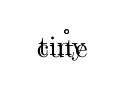
\begin{tikzpicture}[baseline=(current bounding box.north), scale=1.00]
\tikzset{sibling distance=1pt}
\tikzset{every tree node/.style={align=left,anchor=north}}
\Tree [.NP [.{AdjP} \edge[roof];  \node(labelone){cute}; ] [.NP [.{AdjP} \edge[roof];  \node(labeltwo){tiny}; ] [.NP [.SpecNP ] [.{$\overline{\textrm{N}}$} [.{N\textdegree} kitten ] [.{} ] ] ] ] ]
\end{tikzpicture}

\ex \label{ex:kittenadjunctiontreeb}
\begin{tikzpicture}[baseline=(current bounding box.north), scale=1.00]
\tikzset{sibling distance=1pt}
\tikzset{every tree node/.style={align=left,anchor=north}}
\Tree [.NP [.SpecNP ] [.{$\overline{\textrm{N}}$} [.{Adj\textdegree } cute ] [.{$\overline{\textrm{N}}$} [.{Adj\textdegree } tiny ] [.{$\overline{\textrm{N}}$} [.{N\textdegree} kitten ] [.{} ] ] ] ] ]
\end{tikzpicture}


\end{xlist}
\end{multicols}
\end{exe}





\noindent We can immediately rule out the approach in (\ref{ex:kittenadjunctiontreeb}), as it can be shown that adjectives should be regarded as phrases and not as heads as it is possible to replace an adjective with a multi-word expression. For example, it is possible to replace \textit{cute} in \textit{a cute kitten} by \textit{extremely cute} resulting in \textit{an extremely cute kitten}. Additionally, the intermediate-projection adjunction approach is theoretically hard to motivate as ``no other category allows recursive adjunction to an intermediate projection'' \citep[94]{scott2002stacked}. This would lead us to assume that NPs are, in terms of $\overline{\textrm{N}}$ structure, unique -- an undesirable result (see also \citealt{abney1987english}). This leaves us with the possibility in (\ref{ex:kittenadjunctiontree}). However, there is a major problem which, in fact, also occurs with the structure in (\ref{ex:kittenadjunctiontreeb}): adjunction should be free. This means that the order of the adjuncts should play no role (as already argued on page \pageref{generaladjunction}).

So far, we have seen that English exhibits a strict ordering of adjective phrases inside the DP -- a result which is simply an empirical generalization and can hardly be denied. Additionally, it seems as if an adjunction approach is not capable of explaining these restrictions as it would predict the order to be absent. It is thus plausible to assume a rigidly ordered set of (functional) projections as exemplarily shown for the DP \textit{these three beautiful huge old round brown rugs} in (\ref{ex:adjectivetree}). Note that a structure like the one in (\ref{ex:adjectivetree}) simply states that the adjectives are rigidly ordered and says nothing about why this order exists. 




\begin{exe}
\ex \label{ex:adjectivetree}
%\begin{tikzpicture}[baseline=(current bounding box.north), scale=1.00]
%\tikzset{sibling distance=5pt}
\begin{adjustbox}{max width=0.9\textwidth}
\begin{tikzpicture}[baseline=(current bounding box.north),sibling distance=2pt,level distance=45pt
]
%\tikzset{sibling distance=2pt}
\tikzset{every tree node/.style={align=left,anchor=north}}
\Tree [.{{\large DP}} [.{{\large SpecDP}} ] [.{\large{$\overline{\textrm{D}}$}} [.{\large{{D\textdegree}}} {\large{These}} ] [.{\large{NumP}} [.{\large{AdvP}} \edge[roof];  \node(three){{\large{three}}}; ] [.{\large{{$\overline{\textrm{Num}}$}}} [.{\large{{Num\textdegree}}} ] [.{\large{EvalP}} [.{\large{AdvP}} \edge[roof];  \node(beautiful){{\large{beautiful}}}; ] [.{\large{{$\overline{\textrm{Eval}}$}}} [.{\large{{Eval\textdegree}}} ] [.{\large{SizeP}} [.{\large{AdvP}} \edge[roof];  \node(huge){{\large{huge}}}; ] [.{\large{{$\overline{\textrm{Size}}$}}} [.{\large{{Size\textdegree}}} ] [.{\large{AgeP}} [.{\large{AdvP}} \edge[roof];  \node(old){{\large{old}}}; ] [.{\large{{$\overline{\textrm{Age}}$}}} [.{\large{{Age\textdegree}}} ] [.{\large{ShapeP}} [.{\large{SpecShapeP}} \edge[roof];  \node(round){{\large{round}}}; ] [.{\large{{$\overline{\textrm{Shape}}$}}} [.{\large{{Shape\textdegree}}} ] [.{\large{ColorP}} [.{\large{AdvP}} \edge[roof];  \node(brown){{\large{brown}}};  ] [.{\large{{$\overline{\textrm{Color}}$}}} [.{\large{{Color\textdegree}}} ] [.{\large{NP}} \edge[roof]; \node(kaffee){{\large{rugs}}}; ] ] ] ] ] ] ] ] ] ] ] ] ] ] ]

\end{tikzpicture}
\end{adjustbox}
\end{exe}

\noindent According to the Cartographic view, i.\,e., on the assumption that, for example, adjectives are ordered in a fixed set of functional projections, as in (\ref{ex:adjectivetree}), the meaning of the adjectives does not only come from their lexical entries, but is also a function of their syntactic position. What this means is that specific adjective classes (such as evaluative adjectives or size adjectives) are licensed by dedicated functional heads. One interesting piece of evidence that this hypothesis is on the right track is that it is possible for an adjective to receive different interpretations in different positions. This can be illustrated for adjectives which have several readings. An example of such an adjective is \textit{cool} which has a reading as an evaluative adjective meaning `excellent' and a reading as a temperature adjective meaning `not hot' \citep{scott2002stacked}. Although the hierarchies above did not include a TempP so far, we can assume that evaluative adjectives are rather high and temperature adjectives are rather low in the structure -- this is because subjective evaluations seem, in general, to be located rather high in the structure and merely descriptive assesements, such as form, color, or temperature, are located nearer to the noun. This leads us to assume that the adjective \textit{cool} can occupy both positions. And indeed, as \citep[106]{scott2002stacked} illustrates, it is easy to construct examples for both positions as shown in (\ref{coolevaltemp}). Note that the adjective under discussion is in an unexpected position in both examples. 

\begin{exe}
\ex\label{coolevaltemp}\begin{xlist} 
\ex What a long cool red dress. \label{coolevaltempa}
\ex What a cool long red drink. \label{coolevaltempb}
\end{xlist}
\end{exe}

\noindent When putting \textit{cool} in a lower position, as in (\ref{coolevaltempa}), we get the somehow strange reading that the dress that is talked about is not hot, in the sense of cold, i.\,e., a temperature reading.\footnote{ Note that the sentence in (\ref{coolevaltempa}) can additionally be a case in which \textit{long} is preposed by focus movement. However, this is not the kind of structure I am aiming here at.} The sentence, however, does not mean that the dress is excellent. In (\ref{coolevaltempb}), it is the other way around. The adjective is in a high position leading to a reading where \textit{cool} does not refer to the temperature, but to the evaluation of the drink being excellent. Additional support of the idea that different positions license different readings comes from the fact that both readings can be combined, as in \textit{a cool cool drink}.\footnote{ Although such constructions are not widely used due to a general constraint that disfavors phonological similar elements to be adjacent, also known as \textit{horror-aequi} effect.}

So far, it seems as if there is a strict order of adjectives in English. But what about other languages? Interestingly, adjective ordering restrictions seem to be cross-linguistically very stable. We find them, for example, in \is{German}German, \is{Italian}Italian \citep{cinque2010syntax}, \is{Greek}Greek \citep{alexiadou2001adjective}, \is{Finnish}Finnish, the Niger-Congo language \is{Ibibio}Ibibio, Malayalam,\is{Malayalam} \is{Welsh}Welsh \citep{scott2002stacked}, \is{Chinese}Chinese \citep{sproat1991cross}, Taiwan Sign Language\is{Taiwan Sign Language} \citep{zhang2007universal}, or \is{Italian Sign Language}Italian Sign Language \citep{bertone2009syntax, mantovan2017nominalmoditalian}. It thus seems as if the structure of the DP is fixed. In fact, the same pattern that was described for English can be found in DGS. The examples in (\ref{dgsadjectivehier}) illustrate the unmarked order of several classes of adjectives in DGS.\footnote{ Note that with examples with adverbs of origin, like the one in (\ref{dgsadjectivehieracolororiginf}), some signers prefer a PP construction like \textsc{from italy}.}

\begin{exe}
\ex\label{dgsadjectivehier}\begin{xlist} 
\ex \textsc{index}\textsubscript{3a} \textsc{three woman} 
\glt `these three women.' \hfill determininer $>$ number \label{dgsadjectivehiera}

\ex \textsc{three woman beautiful tall} 
\glt `three beautiful tall women.' \hfill evaluation $>$ size \label{dgsadjectivehierb}

\ex \textsc{three church tall old} 
\glt `three tall old churches.' \hfill size $>$ age \label{dgsadjectivehierc}

\ex \textsc{three table old round}%\textsubscript{plural}
\glt `three old green tables.' \hfill age $>$ shape \label{dgsadjectivehierd}

\ex  \textsc{three table round green}%\textsubscript{plural} 
\glt `three round green tables.' \hfill shape $>$ color \label{dgsadjectivehiere}

\ex \textsc{three rug brown italian} 
\glt `three brown Italian rugs.' \hfill color $>$ origin \label{dgsadjectivehieracolororiginf}
\end{xlist}
\end{exe}

\noindent As in other sign languages, e.\,g., in \is{Italian Sign Language}Italian Sign Language (see \citealt[284]{cecchetto2009another}), adjectives naturally occur post-nominally in DGS \citep[18]{herrmann2013modal}, but many signers also allow pre-nominal adjectives (again, similar to Italian Sign Language; this variation is probably due to head movement of the noun). However, the more adjectival signs are used to modify a noun, the stronger the tendency to follow the noun gets (see also \citealt[146]{papaspyrou2008grammatik}). The examples additionally show that while adjectives follow the noun they modify, demonstrative pronouns and numerals precede the NP.

\is{transitivity (method)|)}
Of course, the surface order of the  functional projections discussed so far can deviate from English, as it is easy to see from languages which place their adjectives after the noun, like DGS or \is{French}French (e.\,g., \textit{le tableau noir}, lit. `the table black') and it is indeed not even clear if all languages exhibit adjectives at all, at least in the same way as, for example, English or DGS \citep{croft1991syntactic,dixon2004adjective}. However, the orders that exist can be derived by movement -- and movement operations follow restrictions. From those restrictions, predictions of possible and impossible orders can be made.\footnote{ See \citet[87]{greenberg1963some} who famously stated that when ``any or all of the items (demonstrative, numeral, and descriptive adjective) precede the noun, they are always found in that order. If they follow, the order is either the same or its exact opposite''. } 
And indeed, if we look at the 24 possible orders of demonstratives, numerals, adjectives, and nouns, it turns out that only 14 are attested in the world's languages \citep{cinque2006restructuring,abels2009universal}. This suggests that there are universal restrictions on which order is possible and which is not. The evidence available today suggests that the attested orders are exactly those which can be derived from one basic hierarchical ordering and basic assumptions about movement rules (such as c-command) (see \citealt{medeiros2012movement}). 

Deviant orderings, in any domain, are of special interest, especially when the order in one language is the mirror image of the order in another language. This can be seen, for example, by a comparison of the behavior of demonstratives, numerals, adjectives, and nouns in the Gbe languages \is{Gungbe}Gungbe, illustrated in (\ref{ex:gungbevsenglishadjective}) and English.

\begin{exe}
\ex Gbe \citep[92]{aboh2004morphosyntax} \\
\gll {Àgásá} {ɖàxó} {àtɔ̀n} {éhè} {lɛ́} \\
{crabs} {big} {three} {these} {\textsc{plural}} \\
\trans `These three big crabs.' \label{ex:gungbevsenglishadjective}
\end{exe} 


\noindent When comparing the Gungbe example in (\ref{ex:gungbevsenglishadjective}) to its English translation given in the bottom row of the same example, it is apparent that Gungbe exhibits the order noun--adjective--numeral--demonstrative which is the exact opposite of English. The fact that such mirror images are, by far, not rare cases that occur by chance, but that languages of this sort follow the same strict rules as English (albeit in the inverse way) tells us that there must be some underlying structure -- finding and documenting these structures is the goal of Cartographic syntax.
\is{adjective ordering restrictions|)}

So far, this short introduction to Cartographic syntax was concerned with the structure inside the DP. However, the DP only represents a small portion of the structures syntactitians are concerned with. The largest (self-contained) structure usually playing a role in syntax is the clause. And indeed, applying the transitivity method just introduced to the clause also leads, as I will review in the following chapters, to a rigidly ordered set of functional projections, called the `clausal skeleton' or the `clausal spine'. 

\subsection{The goals of Cartographic syntax}


The Cartographic enterprise has several aims. The chief aim -- at least at the moment -- is to draw a precise map of the projections making up the clausal spine (or other functional projections like the DP, cf. \citealt[3]{cinque2006restructuring}). This endeavor is interrelated with a second aim. Although, by now, there are many Cartographic studies on many languages, it is still unclear which categories are hardwired and which are not. Actually, it is still unclear how many different categories to assume in the structure of the DP or a clause\footnote{ \citep{cinque2010mapping} estimate that there may be more than 400 different functional heads with strict orderings in the clausal domain.} -- and if all projections are always present even if a category is not expressed. This also means figuring out if a specific projection exists in languages that do not have any means to express this category in a grammaticalized way. Another goal of Cartography, on which not much light has been shed so far, is to figure out the source of the strict ordering of functional categories and how they came into being. However, this can only be achieved when it is fully clear how such maps, the Mendeleev tables of syntax \citep[199]{rizzi2013notes}, so to speak, will look like:

\begin{quote}
It is obvious that if we raise questions about such issues as $[$\dots $]$ ``the $[$\dots $]$ basis of X,'' or ``the origin and evolution of X,'' without knowing the essential properties of X $[$\dots $]$, then we will only have, at best, very vague and unrevealing ``answers'' to the questions. \citep[8]{fukui2004tro}
\end{quote}

\noindent Before asking why there is a multitude of strictly ordered functional projections, how this strict ordering came into being, or if these orderings are part of an innate UG or if they can be derived by third factors,\is{third factor principles} it seems plausible to figure out their exact shape and properties -- nevertheless, the question of how cross-linguistically stable ordering restrictions arose has bothered linguists questioning the relation between Cartography and Minimalism, as described next.

\subsection{Cartography and Minimalism: UG or third factor principles?}
\is{third factor principles|(}
%Cartography and Minimalism
\noindent While at first Cartographic and Minimalist accounts of syntax seem to contradict each other, both should not be seen as excluding, but rather complementing each other. While modern Minimalism (e.\,g., \citealt{chomsky2005three}) tries to argue for a minimal role of innate linguistic structures (i.\,e., Universal Grammar) stressing the role of factors of general cognition (so called `third factor principles'), the cartographic approach (e.\,g., \citealt{cinque1999adverbs}) favors the idea of an extremely rich inventory of universally available syntactic projections. Both positions are equally plausible, but taking either of them seriously leads to unsolvable problems for the other:

\begin{quote}
Taking the Minimalist Program seriously, we are forced to reject the rich functional hierarchy as an axiomatic part of UG; there is no plausible evolutionary scenario to support the natural selection of a language faculty with such a highly structured organization of functional categories. \citep[172]{ramchand2014deriving}
\end{quote}

\noindent The other way around, however, ``taking the results of the Cartographic enterprise seriously, we are forced to seek a source for the rich functional hierarchy'' (ibidem). The solution of Ramchand \& Svenonius is that both positions are right. On the one hand we should follow the Minimalist idea of a minimal role of UG, but on the other hand we cannot ignore the massive uniformity of the strict ordering of functional categories as it is a cross-linguistically stable empirical fact. What linguistics thus should do is to look for extralinguistic sources of the functional hierarchy:

\begin{quote}
It is hard to imagine that the hierarchy may be an irreducible property of UG, disconnected from any other aspect of human cognition; it is also hard to believe that the hierarchy may be a purely arbitrary ``cultural'' property, rediscovered by every language learner in the same form, language after language, on the basis of pure inductive learning. So, there must be some principles determining the hierarchical sequence, and guiding the child to ``rediscover'' it in the course of language acquisition. \citep[52]{cinque2008cartography}
\end{quote}

\noindent Before introducing sign languages and their structures in the next section, I briefly want to mention one last property of the structural make-up of clauses, namely, that not all categories need to be cross-linguistically ordered. One major example of a category which is known to float is negation. The structural position of negation, often assumed to be located in a NegP, seems to be subject to variation not only cross-linguistically, but sometimes also within a single language (e.\,g., \citealt{ouhalla1990sentential, ouhalla1991functional}; \citealt{zanuttini1991syntactic}). Thus Cartography also needs to figure out why some categories are strictly ordered and why others are variable.

\is{third factor principles|)} 



\section{Hypotheses}\label{hypotheses}
The main goal of this book is two-fold. On the one hand, it presents an introduction to the general clause-structure of German Sign Language. On the other hand, it seeks to test several hypotheses which can be derived from what I call \is{bodily-mapping hypothesis}`the bodily-mapping hypothesis', originally proposed in \citet{bross2017scope}. In this section, I will briefly review the main claims made in \citet{bross2017scope} and extend their hypotheses. % and then discuss how these claims will be explored in the following chapters.

There seems to be a general division of labor between the non-manual markers of the upper and lower face with the upper-face non-manuals spreading over larger domains fulfilling syntactic functions and the lower face being associated with smaller spreading domains fulfilling adjectival/adverbial functions (see also Figure \ref{upperlowerfacedivisionoflabour} on page \pageref{upperlowerfacedivisionoflabour}). While the difference in spreading domain of upper and lower face has mainly been an alignment claim so far, the hypothesis that non-manuals produced with higher articulators have a more broad scopal domain and those produced with lower body parts have a more narrow scopal domain can be easily deduced by this finding (see also the quote from \citealt[249]{wilbur2009productive} cited on page \pageref{wilburquote}). 

In fact, this claim can be brought to the extreme by hypothesizing that the fixed scope order of clausal categories is directly mapped onto the body in sign languages. To be more precise, higher scoping categories are expressed by physically higher articulators and lower scoping categories are expressed by physically lower articulators. This is basically the claim made in \citet{bross2017scope}.

\subsection{A Typology of Scope-Taking Strategies}
\citet{bross2017scope} distinguish two basic means of expressing scopal relations. Scope is either expressed by layering or by concatenation. With layering, the scope-taking element and its scope are expressed simultaneously. This can be exemplified by comparing English assertions and yes/no-questions (in form of raising declaratives), as in the minimal pair in (\ref{fuenfzehn}), from \citet{bross2017scope}.

\begin{exe} 
\ex \label{fuenfzehn}
\begin{xlist} 
\ex 
\gll {} {\hspace{12pt} HL L} \\
She departed. \\ \label{fuenfzehna}
\ex 
\gll {} {\hspace{12pt} HL H} \\
She departed? \\ \label{fuenfzehnb} 
\end{xlist} 
\end{exe}

\noindent The example shows two sentences with identical lexical material only differing in intonational contours (H stands for high tone and L for low tone). The fact that (\ref{fuenfzehna}) is understood as an assertion and (\ref{fuenfzehnb}) as a question is only due to the supresegmetal layer of intonation that is added `on top' of the lexical items. Thus, the speech-act operators are said to be layered. 

However, scope can also be expressed by linearization. There are two options for linearly expressed operators to express scope in terms of sequencing. Either an operator takes scope over the material following the operator or it takes scope over the material preceding it. These two options are summarized in (\ref{beispielvierzehn}), from \citet{bross2017scope}.

\begin{exe} 
\ex \textit{Sequencing of operators and scope-taking} \label{beispielvierzehn} 
\begin{xlist} 
\ex 		O $>$ P \\ `If operator O is pronounced before operator P, then O takes scope above P.' \label{beispielvierzehna}
\ex P $<$ O \\ `If operator O is pronounced after operator P, then O takes scope above P.' \label{beispielvierzehnb} 
\end{xlist} 
\end{exe}

\noindent In the first case, we can, metaphorically, say that scope-taking proceeds from left to right and in the second case from right to left (with `right' and `left' as metaphors for preceding and following). Both strategies, i.\,e., left-to-right and right-to-left concatenation, are found in natural languages. This can be illustrated by comparing English, a VO language, with German, an OV language. At least concerning some portions of the clause, English and German are mirror-images of one another, as English employs a  left-to-right concatenation strategy while German employs a right-to-left concatenation strategy, as shown in (\ref{droelf}), again from \citet[11]{bross2017scope}, for the categories of epistemicity, tense, and root modality (with epistemic modals taking highest and root modals taking lowest scope).\footnote{ Note that the example is a bit of a oversimplification as \textit{have}/\textit{haben} does in fact not represent Tense, but is an instance of perfect. However, nothing hinges on that as the example only serves illustrative purposes. For a similar phenomenon compare example (\ref{ex:gungbevsenglishadjective}) on page \pageref{ex:gungbevsenglishadjective} concerning adjective orders.\is{Gungbe} In this case, the order of adjective in Gungbe was the mirror image of the order of adjectives in English.}

\begin{exe} 
\ex \label{droelf}
\begin{xlist} 
\ex 	\dots\ because Paula must$_{\text{EPISTEMIC}}$ have$_{\text{TENSE}}$ been able$_{\text{ROOT}}$ to repair her bike.\label{beispieldreizehna}
\ex \gll \dots\ weil Paula ihr Fahrrad reparieren gekonnt$_{\text{ROOT}}$	haben$_{\text{TENSE}}$ muss$_{\text{EPISTEMIC}}$. \\
because Paula	her	bike		repair			been.able	  	have			must \\
\glt `\dots\ because Paula must have been able to repair her bike.'
 \label{beispieldreizehnb} 

\end{xlist} 
\end{exe}

\noindent It has to be noted that natural languages often do not uniformly employ either a left-to-right or a right-to-left concatenation strategy, but have switches. As can be seen in the German sentence in (\ref{beispieldreizehnb}), for example, the complementizer \textit{weil} `because' (a syntactic head), being structurally extremely high (in the CP domain) is concatenated from left to right (and not from right to left). Thus, at some point in the syntax (between the CP and the IP) there must be a pivotal point at which the strategy switches. 

\subsection{Scope mapped onto the body}
So far, the two strategies, layering and concatenation, were introduced using examples from spoken languages, but they easily map onto sign languages as well. Layering is realized by the simultaneous expression of lexical materials (i.\,e., manual signs) and non-manual markers while concatenation simply is realized by the temporal sequencing of manual signs. The general hypotheses constructed in \citet[14]{bross2017scope} concern the three different strategies of expressing scopal relations (i.\,e., layering, left-to-right, and right-to-left concatenation) and the height/width of the scope of an operator:



\begin{exe} 
\ex \label{hypohypo} 
\begin{xlist} 
\ex \textit{High body parts for comprehensive operators} \\
The wider/higher the scope of an operator is, the more likely it will be expressed by layering with a body part that can be ordered relative to other expressions on a vertical axis. In this way, a relatively wide/high scope correlates with a relatively high body part.   \label{hypothesisa}
\ex \textit{Left-to-right concatenation for operators with intermediate scope}\\
Intermediate operators are produced with a manual left-to-right concatenation strategy.  \label{hypothesisb} 
\ex  \textit{Right-to-left concatenation for least comprehensive operators} \\
The lower/narrower the scope of an operator is, the more likely it will be expressed by way of a manual right-to-left concatenation strategy. \label{hypothesisc}
\end{xlist} 
\end{exe}


\begin{figure}[bt]
\centering
	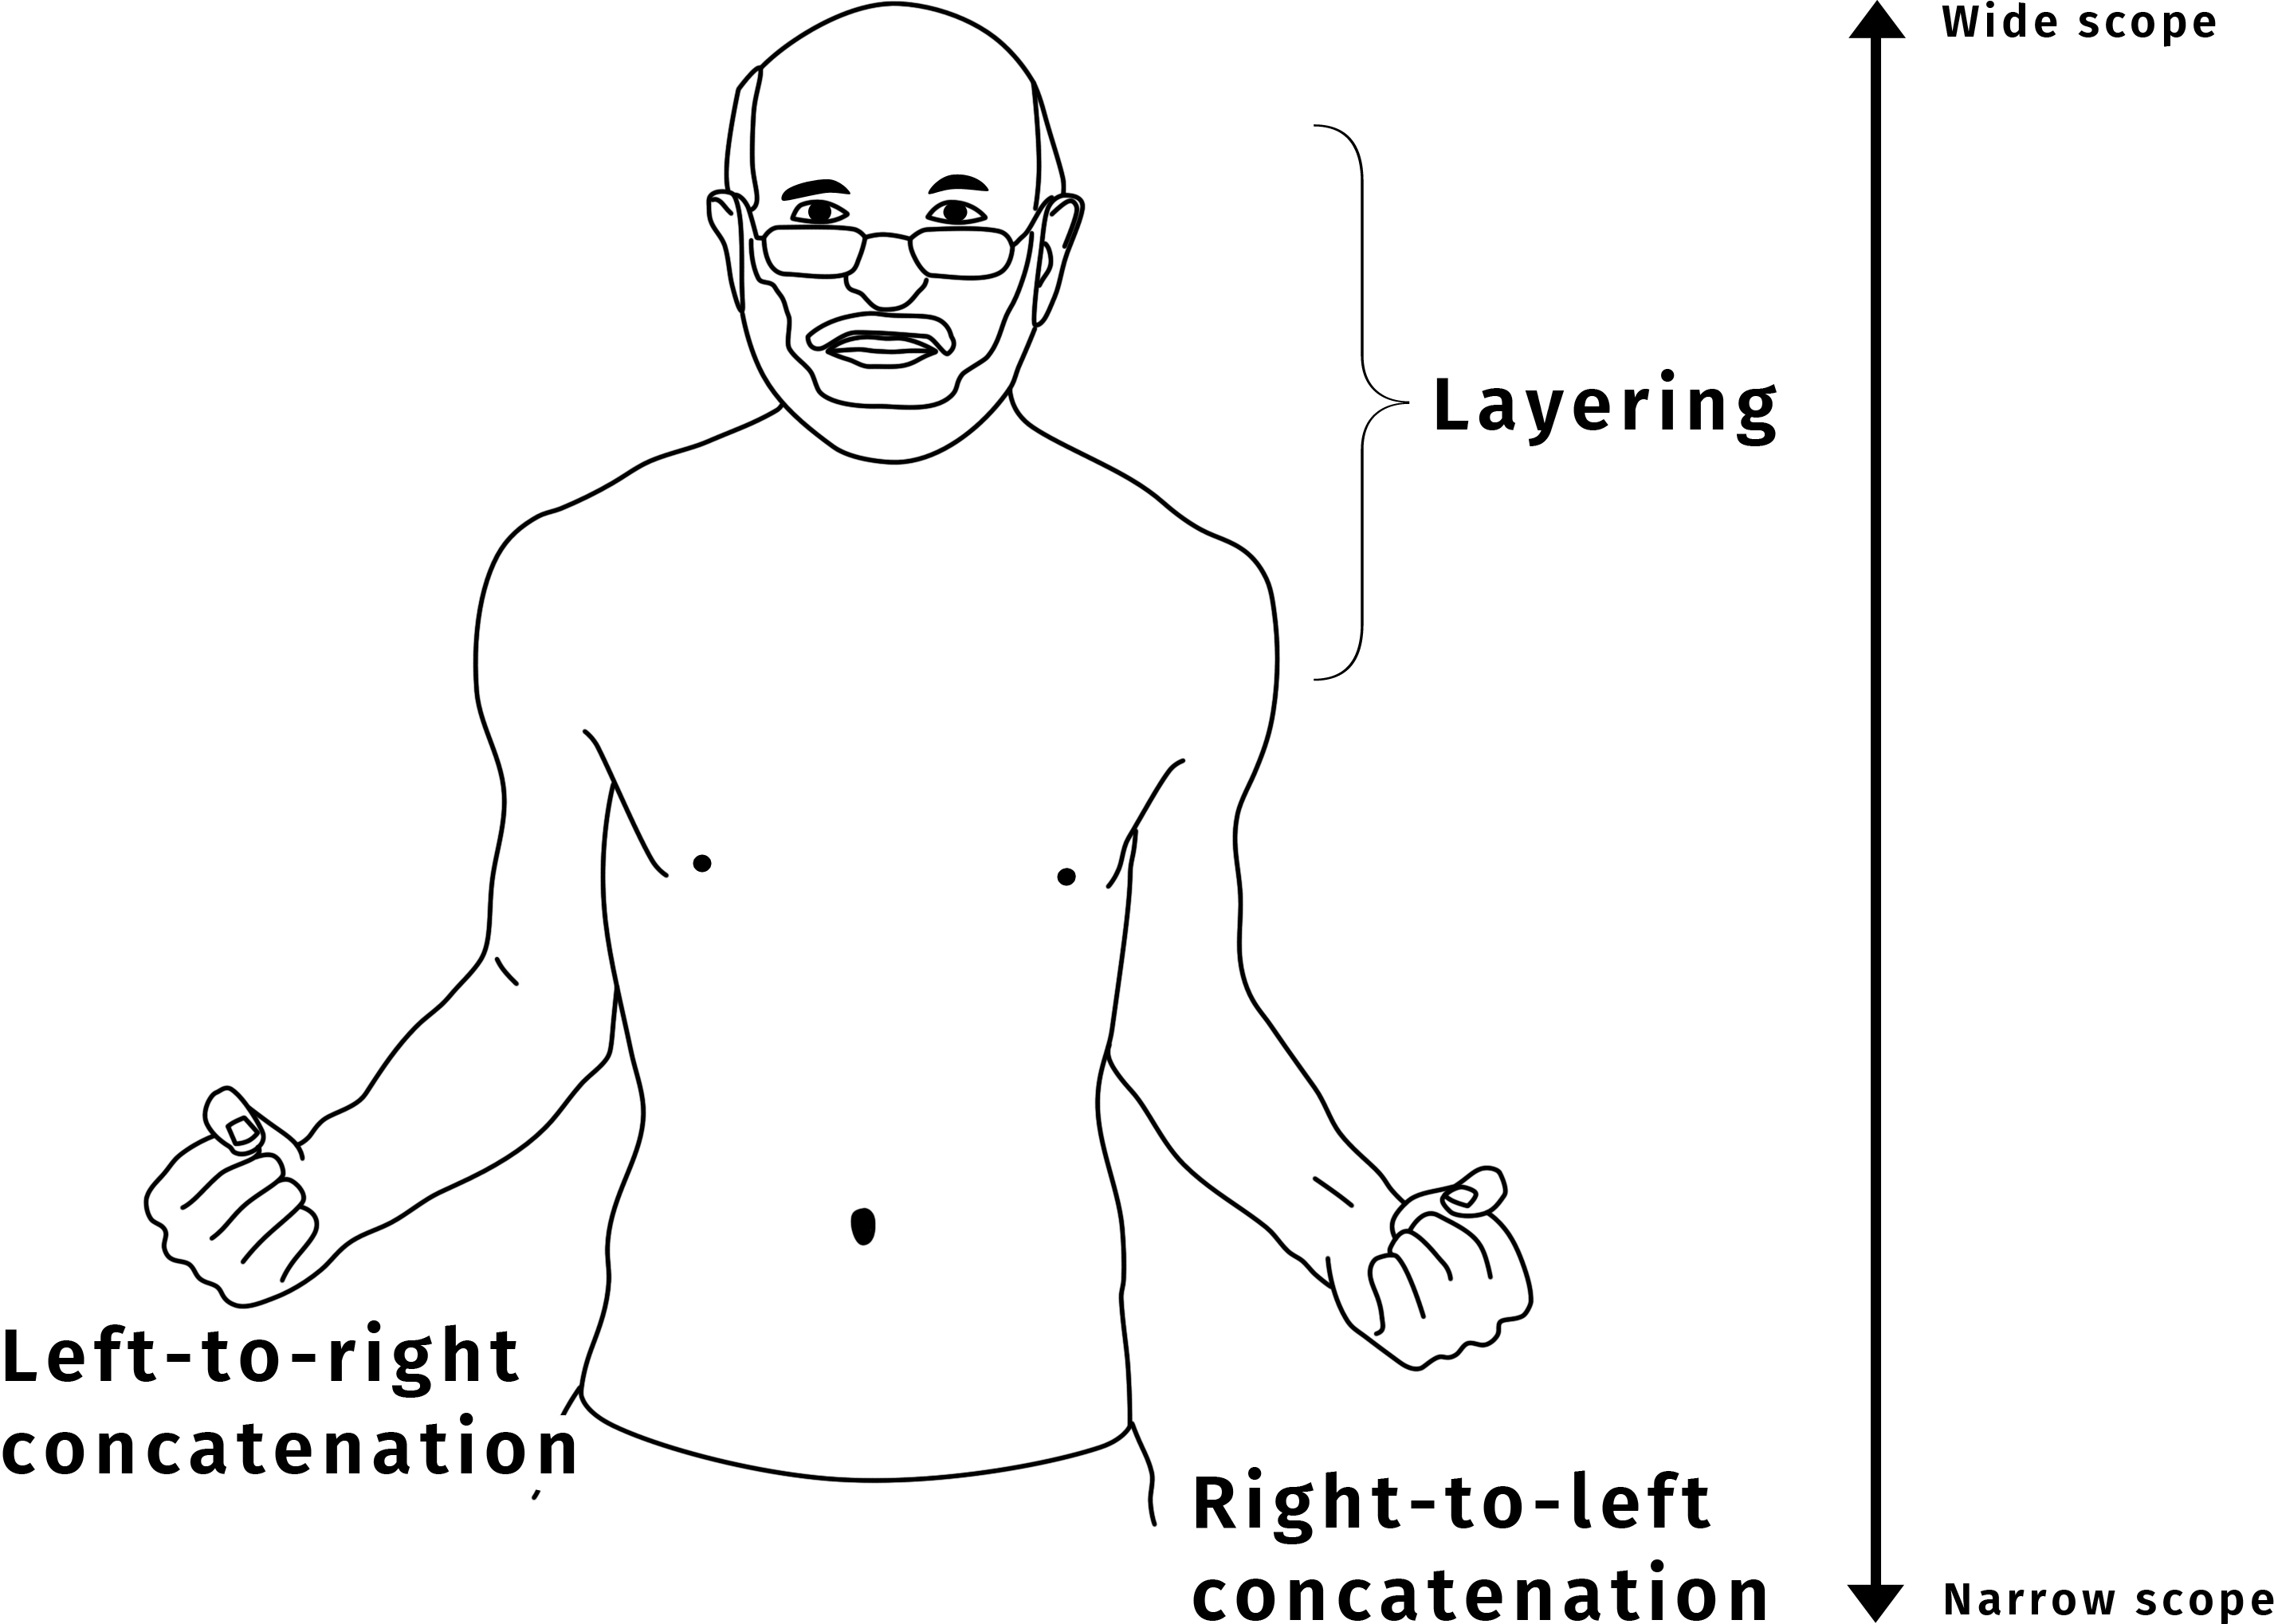
\includegraphics[width=1.0\textwidth]{hyposw.jpg}
	\caption{The main hypotheses by \citet{bross2017scope}: Scope is directly mapped onto the signer's body (called the \is{bodily-mapping hypothesis}bodily-mapping hypothesis). The higher the scope, the liklier a category will be expressed via layering and the higher the scope, the higher the articulator. At some point in the syntactic tree, scopal relations are expressed via concatenation, first from left to right, then switching to right to left. The two concatenation strategies are metaphorically depicted as the left and the right hand -- although `left' and `right' refers to the relative sequencing of manual signs in time and not to the left or right hand.}
	\label{hypo}
\end{figure}	

\noindent It has to be noted that the vertical mapping of scope proposed by Bross \& Hole does not concern the place of articulation of a manual sign which can be high or low on the body (e.\,g., the forehead versus the abdominal region), but only concerns the articulators themselves. Another important note relates to the fact that there are articulators in sign languages for which it is unclear how high they actually are. It is, for example, clear that the eyebrows are located above the mouth, that the mouth is above the shoulders and that the shoulders are above the hands. If a signer, however, tilts her/his head back, it is rather unclear if the head should be taken to be higher than, lets say, the mouth:\footnote{ There are, of course, many functions fulfilled by movements of, for example, the whole head. As an anonymous reviewer correctly pointed out, single head movements are often observed with focus and repeated head movements (nods) with affirmative functions: This could lead to the speculation that domain marking (repeated nods) and punctual marking (single nods) can also be used to indicate syntactic height. Another hypothesis worth investigating may be the head movements in general are related to truth values. Typical functions which involve movements of the head are negation (head shake), affirmation (repeated nodding), contrastive focus (see Section \ref{contrastivefocussubection}), or epistemic commitment (see Section \ref{polarinterrogativesdgs}).}\label{nesting}

\begin{quote}
A problem to be solved is the question of mereological nesting: Is a body part as a whole, when it performs an action, higher than a subpart of this body part? Is a nodding head, for instance, higher than raised eyebrows or lower? It may turn out that such issues can be resolved empirically by investigating what kind of visual information signers rely on when observing the respective movements. For example, it may turn out that the critical point to evaluate how a nod is perceived is the position of the tip of the nose. If this was the case, then one could convincingly argue that a nod is lower than the eyebrows. \citep[24]{bross2017scope}
\end{quote}

\noindent In the remainder of the book I will mainly concentrate on articulators for which it can be clearly stated that one is above another and exclude claims about the head -- at least when it comes to scope-taking. The main hypotheses are depicted in Figure \ref{hypo} (Figure adapted from \citealt[25]{bross2017scope}).

The figure shows that it is assumed that categories taking high scope (i.\,e., CP categories) are expressed via layering. At the same time, descending the hierarchical ordering of clausal categories means descending the body (the bodily-mapping hypothesis). The highest-scoping categories are expressed with the eyebrows and eyes, lower categories with the cheeks and the mouth and even lower categories with the shoulders. Finally, at some point, the strategy switches from layering to concatenation -- in German Sign Language, first left to right, then right to left (with left to right for higher and right to left for lower categories). Note that this does not mean that signers use their right or left hands. This is only a metaphorical depiction of sequential ordering of manual signs in time (i.\,e., either O $>$ P or P $>$ O), cf. (\ref{beispielvierzehn}) above. Additionally, note that the claim that the switching from non-manual to manual articulators starts with a left-to-right strategy and then changes to right-to-left is a claim for DGS, while the bodily mapping hypothesis is a claim concerning all sign languages. 

That scope is mapped onto the body in a way that could even be called iconic is, by far, not a necessity (cf. the excursus on iconicity). Quite the contrary: it would be rather plausible to assume that a language in the visual modality would express concrete concepts and not abstract syntactic relations in a truly iconic way. Take the concept of smiling. A sentence like \textit{Marla smiled} could easily be depicted by signing the name sign for Marla and finally performing a smile, as shown in (\ref{ex:smilingexamplea}). However, this is not what we find -- neither in DGS nor in any other sign language I am aware of. Instead, the sign for smiling is a manual sign, as shown in (\ref{ex:smilingexampleb}).

\begin{exe}
\ex\label{smilingexample}\begin{xlist} 
\ex \slg{*marla} \slg[smile]{\textcolor{white}{smile}}
%\ex {} {\hspace{41pt}smile}   \\
%{*\textsc{paul}} {$\overline{\textrm{\textsc{\textcolor{white}{smile}}}}$} 
\glt \textcolor{white}{*}`Marla smiled.' \label{ex:smilingexamplea}
\ex \textcolor{white}{*}\textsc{marla smile}  
\glt \textcolor{white}{*}`Marla smiled.' \label{ex:smilingexampleb}
\end{xlist}
\end{exe} 
%

\begin{digression}{Iconicity and the bodily-mapping hypothesis}{}\label{iconicity}
\is{iconicity|(}
\noindent Earlier I claimed that the hypothesized mapping of scope onto the body could be called iconic. As iconicity is often understood as a transparent relation between a concrete meaning and form at a morphological, lexical, or syntactic level, and not as a mapping between an abstract meaning (scope) and form (the body), I will make some brief remarks on the term as it is used here. \citet[20]{taub2004iconicity}, for example, notes that with iconic items, ``some aspect of the item's physical form (shape, sound, temporal structure, etc.) resemble a concrete sensory image''. The problem with this definition is that it is constrained to an ``item's physical form'' and thus excludes more abstract uses of the term. For this reason, I will adopt a broader definition of iconicity based on \citet{jespersen1922language} and \citet{jakobsonwaugh1979soundshape}. \citet[396]{jespersen1922language} defines iconicity (or sound symbolism)  as ``a natural correspondence between sound and sense''. Similarly, \citet[178]{jakobsonwaugh1979soundshape} define it as ``a natural similarity association between sound and meaning''. Of course, this definition, again, is too narrow as it is constrained to sound. 

If we take the organization of the clausal spine as `natural' in a way that it is (presumably) shared by all languages and if we take iconicity to be `a natural similarity association between linguistic form and meaning' the bodily-mapping hypothesis states that sign languages iconically map syntactic structures onto the body. There are two more notes to make. First, the similarity between syntax and the body lies in the fact that both are organized in a hierarchical way. Thus, structures located higher up in the clausal spine take scope over lower structures. Similarly, articulators in sign languages located higher up on the body take scope over expressions encoded by lower articulators. The second note concerns the term `meaning'. As this term is used in a fairly broad sense here, I will clearly state which kind of meanings we are concerned here: As iconicity is understood as a relationship between form and meaning, the bodily-mapping hypothesis is an hypothesis about the height or an articulator (the linguistic form) and the height (or: width) of the scope an operator takes (meaning).

Iconicity, of course, usually relates a linguistic form to an extra-linguistic meaning. In this case, however, it is a linguistic form that relates to a linguistic meaning. In this way, the iconicity of the proposed mapping principle is different from many cases of iconicity discussed in the linguistic literature.


\is{iconicity|)}


\end{digression}

\noindent There seems to be no possibility to express lexical concepts via facial articulators (only) in sign languages. Instead, manual sign must be used, although the signs for concrete actions like smiling or crying indeed have their places of articulation in the face. 

If Bross \& Hole's hypotheses are correct, this will mean that neighboring categories will find similar expression. I call the principle that neighboring categories, i.\,e., categories which are adjacent in the syntax, find similar expression in a language the `principle of analogical designation' (see the following excursus).\footnote{ For a similar observation regarding syncretism in the case hierarchy, see \citet{caha2009nanosyntax} and for compounding see \citet{hole2015arguments}.}

\begin{savenotes}
\begin{digression}{The Principle of analogical designation}{}
\is{analogical designation|(}
\noindent What\label{analogicaldesignation} can be derived from the observations made by \citet{bross2017scope}, if they are indeed correct, is that neighboring categories on the Cinquean hierarchy (introduced in detail in Chapter \ref{ipsystem}) are expressed in similar ways, i.\,e. by using adjacent body parts: the nearer two categories are in the hierarchy, the nearer their expression will be on the body. I call this idea that syntactic proximity is mirrored by phonological similarity the `principle of analogical designation'. We find similar ideas all over the history of linguistics. Otto Behaghel, for example, famously stated that elements which belong close together conceptually will also be placed close together in a sentence.\footnote{ \, The original quote reads ``Das oberste Gesetz ist dieses, da\ss\ das geistig eng Zusammengehörige auch eng zusammengestellt wird'' \citep[4]{behaghel1932}.} While Behaghel's First Law is concerned with the placement of words and phrases in clauses, the principle of analogical designation is concerned with the expression of grammatical categories \textit{per se}. It thus resembles more Wilhelm von Humboldt's observation that related concepts are likely to be expressed phonologically similar cross-linguistically: ``Since \textit{words} always correspond to \textit{concepts}, it is natural for \textit{related concepts} to be designated by \textit{related sounds}.''\footnote{ \textcolor{white}{n}The original quote reads: ``Da \textit{Wörter} immer \textit{Begriffen} gegenüberstehen, so ist es natürlich, \textit{verwandte Begriffe} mit \textit{verwandten Lauten} zu bezeichnen.'' \citep[75]{von1836kawi}. Note that Humboldt also explicitly uses the word `analogy' when talking about ``designation'' and an ``analogy of concepts and sounds'' (the German original: ``Man kann diese Bezeichnung, in welcher die Analogie der Begriffe und der Laute\dots\ die \textit{analogische} nennen'' \citealt[81]{von1836kawi}; the English translations were taken from \citealt{humboldt1999language}). All emphases in original. } The general idea of the principle of analogical designation can be compared to the Nanosyntactic *ABA theorem stating that only adjacent categories can undergo syncretism (see, for example, \citealt{bobalji2007comparative,bobalji2012universals,caha2009nanosyntax}.)

While I will shed some light on the principle of analogical designation in the course of this book, there is much more work to do. It sometimes seems as if the expression of some categories can jump over larger portions of the tree, although not completely random: Many languages, for example, use the same modal verbs to express different kinds of modality (e.\,g., epistemic or deontic modality). Suppose we have three different kinds of modality, A, B, and C hierarchically ordered as A $>$ B $>$ C. While I would propose that it is unlikely that a language uses the modal verb x to express A and C, but another modal to express B, as this would violate the principle of analogical designation, it is unclear why the principle should hold in the first place as there are many other grammatical categories intervening between the different modalities which do not find similar expressions. 

\is{analogical designation|)}
\is{principle of analogical designation|see{analogical designation}}

\end{digression}
\end{savenotes}

\noindent While \citet{bross2017scope} have found evidence that the high-scoping speech-act operators (indicating that a clause is to be understood as a question, an imperative, etc.), the evaluation as good or bad, and epistemic modality are expressed non-manually with upper-face articulators in DGS, \is{scalarity}scalarity (the evaluation as being much or little, see \citealt{hole2015distributed}) is produced non-manually with the lower face. Additionally, they have shown that even lower categories -- those below tense --, like volition, deontic, and root modality are produced manually only. While they take volition to be expressed by employing a left-to-right-concatenation strategy, they claim that root modals concatenate from right to left -- while deontic modals seem to allow both strategies and, thus, present an unclear picture (for an exact description of why some of these categories are higher and others are lower see Chapter \ref{ipsystem}).

An additional claim by \citet{bross2017scope} was that the general split between categories above and below tense is not only a split between layering and concatenation, but also a semantic split between meanings which do not directly contribute to truth conditions (not-at-issue meaning) and meanings which do contribute to truth conditions (at-issue meaning) (see \citealt{simons2010projects, tonhauser2013toward}). This claim has far reaching theoretical consequences as it is not a purely semantic claim, but a syntactic one as it states that the at-issue/not-at-issue divide is hardwired into syntax: not-at-issue meanings are the meanings expressed by the categories above tense, while at-issue meaning is the meaning contributed by the categories below tense. This hypothesis is restated in (\ref{atissuenotatissuedivide}).

%%%%%%%%%%%%%%%%
\clearpage
%%%%%%%%%%%%%%%%

\begin{exe}
\ex \textit{The at-issue/not-at-issue divide hypothesis} \\
The split between categories expressing not-at-issue and at-issue meanings is hardwired into syntax: Categories above tense are not-at-issue while categories below tense are at-issue.\label{atissuenotatissuedivide} In sign languages, this split finds visible effects as categories above tense find their expression via non-manual markings and categories below tense are marked manually.
\end{exe}

\noindent I will discuss this hypothesis in more detail in Section \ref{atnotissue} where I will review some DGS data and show that non-manual expressions indeed always contribute not-at-issue meanings. 

While \citet{bross2017scope} only looked at some clausal categories, this book is an attempt to broaden the picture by investigating the whole range of clausal categories in the CP, IP/TP, and VoiceP domain and put their claims to test (with VoiceP being the highest verbal layer introducing the agent in its specifier). For this reason this book is organized into three main chapters, one devoted to each of the three clausal layers. 

Beside the four main claims, (i) the \is{bodily-mapping hypothesis}bodily-mapping hypothesis in the narrow sense, (ii) that categories below tense are expressed by a manual left-to-right-concatenation strategy, that (iii) even lower categories are expressed by a right-to-left concatenation strategy, and (iv) the at-issue/not-at-issue divide hypothesis, I hypothesize that lower aspectual categories which modify the event itself are again expressed by layering, but by a special form of layering I call `lower layering' or `inner layering'.\is{lower layering}\is{inner layering|see{lower layering}} To be more precise, I observe that aspectual categories below VoiceP are expressed by manipulating the movement path of the verb sign (i.\,e., there is a simultaneous expression of the verb and an aspectual category):

\begin{exe}
\ex \textit{The VoiceP-internal modulation hypothesis:}\is{VoiceP-internal modulation hypothesis}\\
Aspectual categories below the VoiceP (the so-called `inner aspects')\is{inner aspect} do not find their expression by adding manual signs, but by modulating the movement path of the verb sign. \label{vpinternalmodhyp}
\end{exe}

\noindent This hypothesis will be put to test in the IP and VoiceP parts of the book (i.\,e., Chapters \ref{ipsystem} and \ref{insidevp}). Taken together, there are five guiding hypotheses which will be put to test while going through the clause structure of German Sign Language throughout the book. In summary, the proposal looks as in (\ref{treeovervies}) (see next page). The tree shows the basic structure of DGS, following the basic assumptions presented in Section \ref{basicclausstructuredgs} (all heads are final for now) extended by the higher and lower aspectual categories described in \citet{cinque1999adverbs, cinque2006restructuring}. Note that the tree only shows the highest outer and inner aspects. The complement branches of the two aspects are dotted to indicate that other aspectual categories are left out.




The tree depicts the assumption that the higher categories will be expressed by way of layering, while the higher, IP-internal aspectual categories (called `outer aspects') find manual expression and the lower aspectual categories (the `inner aspects')\is{inner aspect}, located below VoiceP find their expression by modulating the movement path of the verb sign (probably, the verb moves into the corresponding aspectual projection in the case of inner aspect). 

\begin{exe}
\ex\label{treeovervies}
\begin{minipage}[t]{\linewidth}
          \raggedright
          \adjustbox{valign=t}{%
            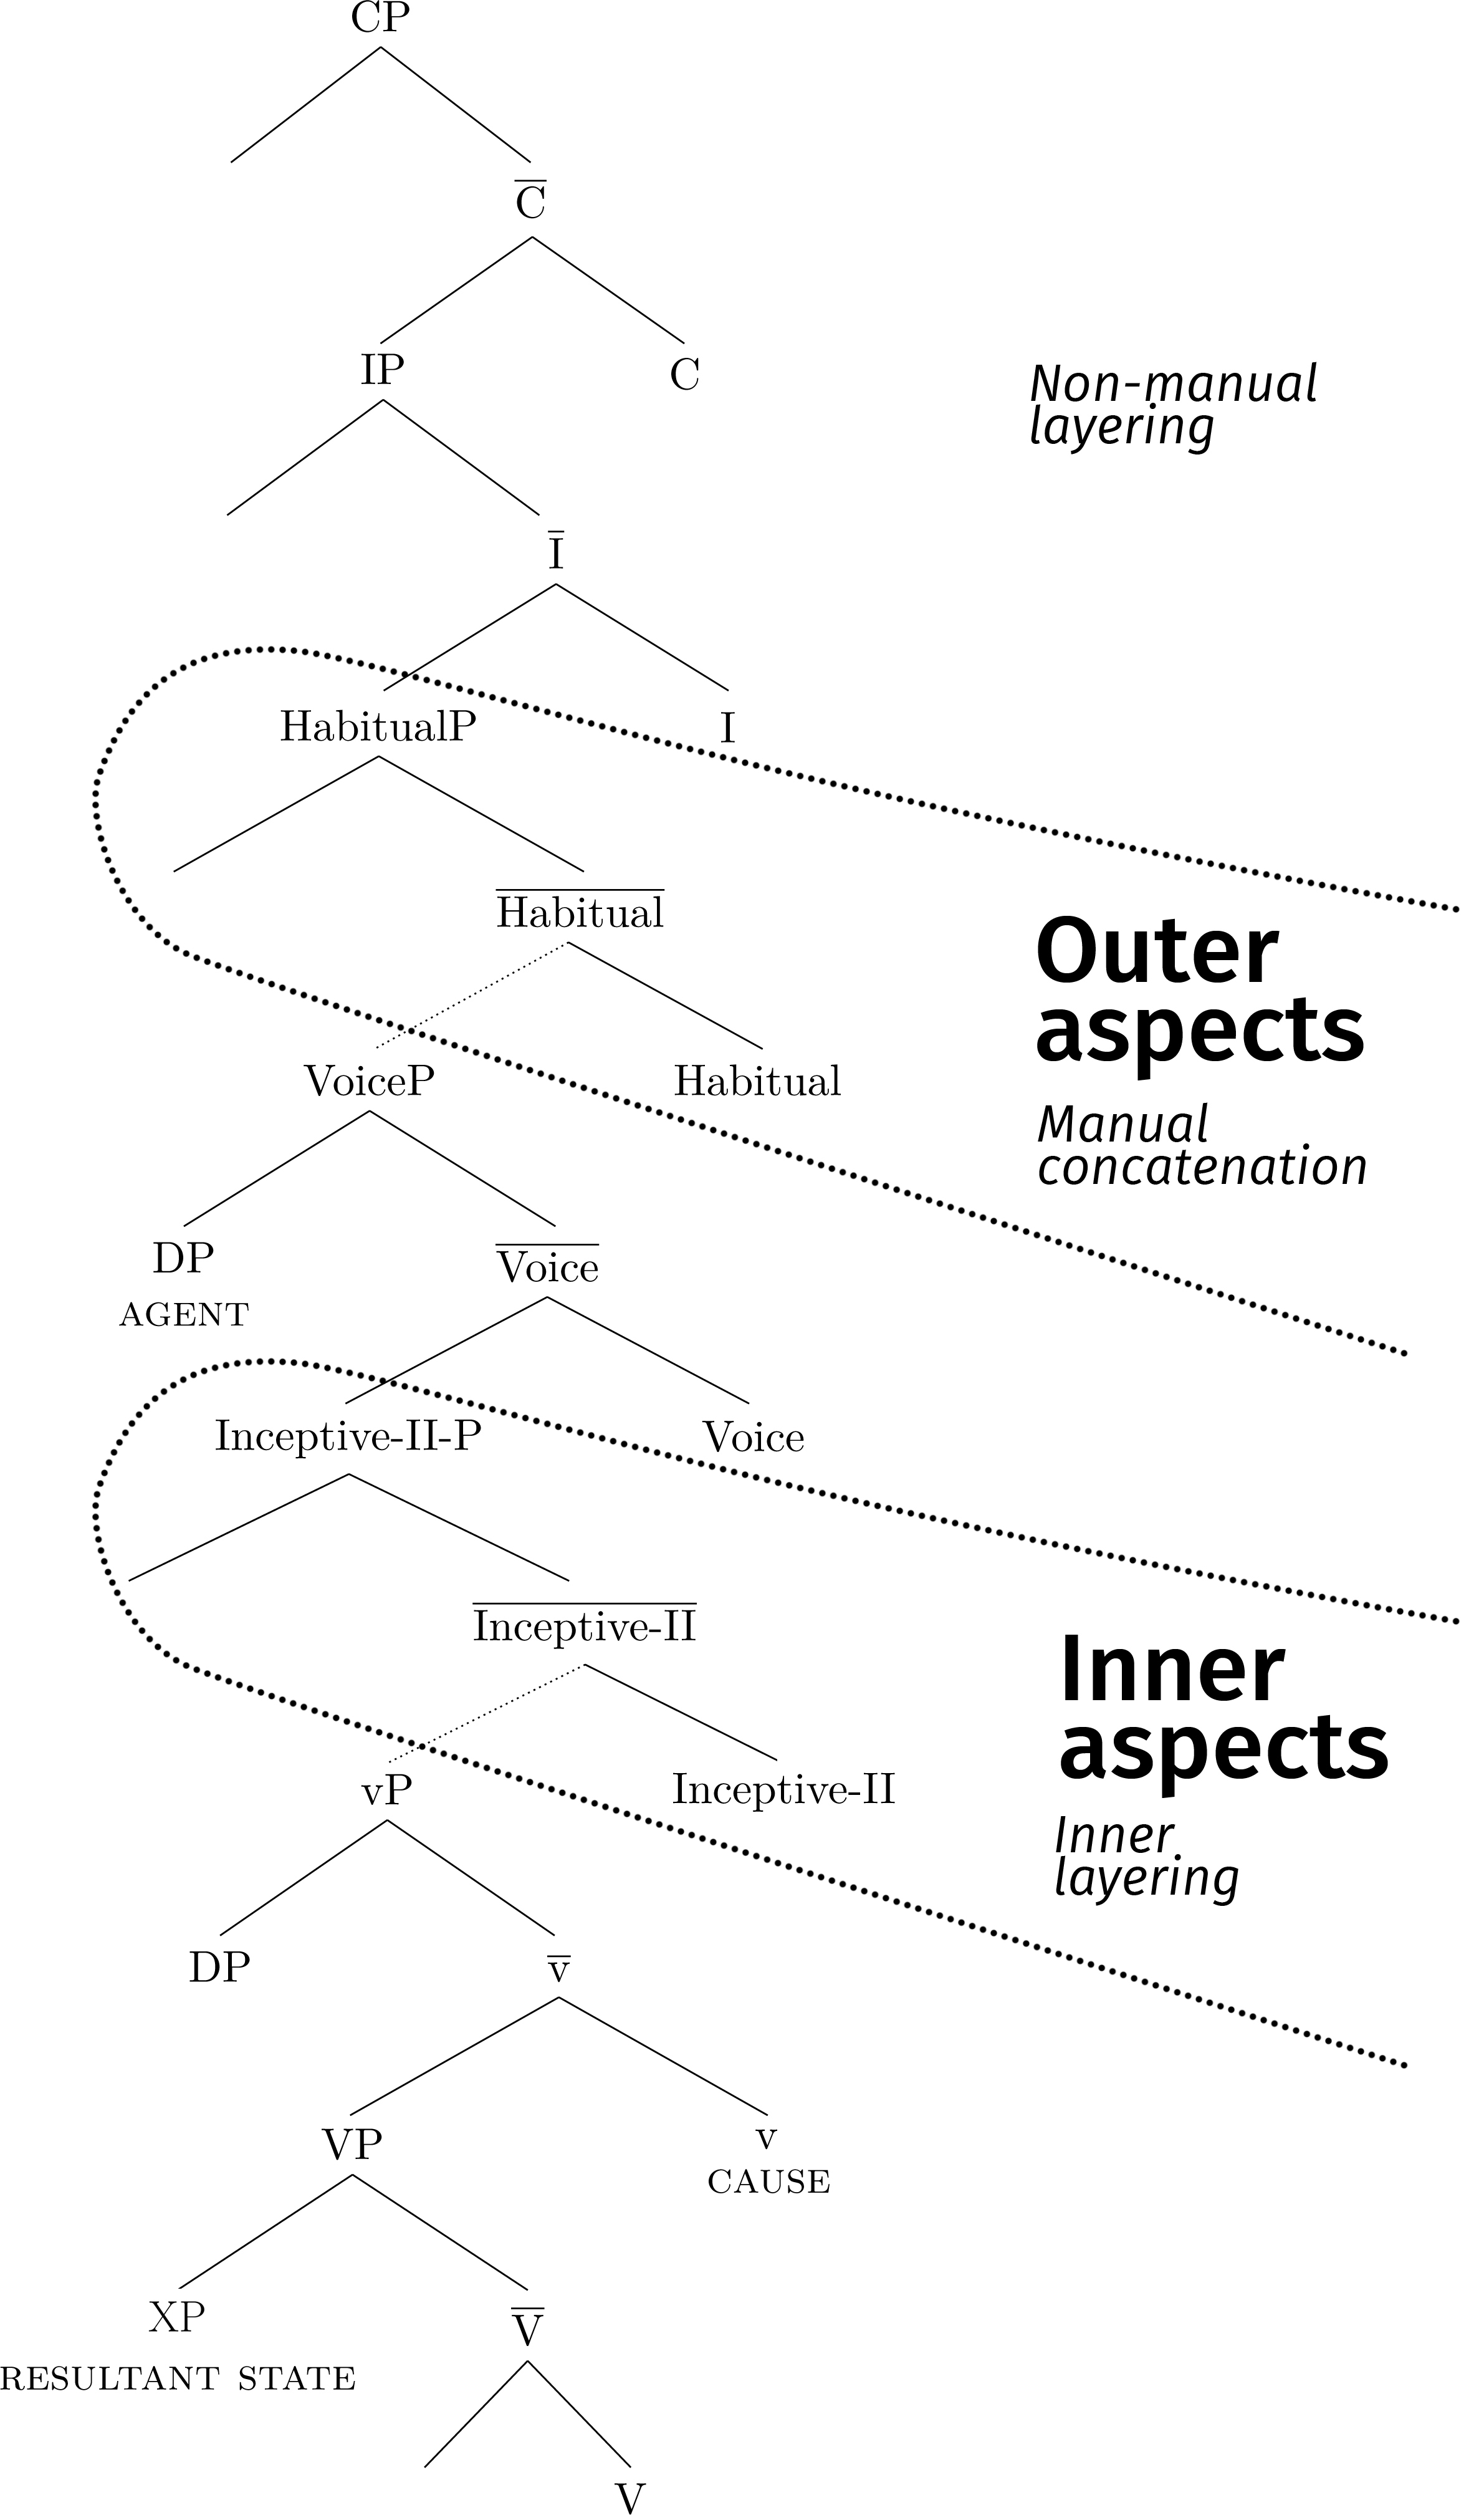
\includegraphics[width=0.7\linewidth]{treesw.jpg}%
          }
    \end{minipage}
\end{exe}










